\section{Deep Stream}
This section presents the performance evaluation of the proposed two-stage people counting system. The primary metric for assessment is Frames Per Second (FPS), which indicates the system's throughput and its capability for real-time processing. We will analyze the FPS at key points in the pipeline: the processing on the NVIDIA Jetson device.
\subsection{Experimental Setup}
{Window Host Configuration}:
\begin{itemize}
    \item GPU: NVIDIA GeForce RTX 4060 Ti
    \item RAM: 32GB DDR5
    \item SR model: WaveMix.pth
    \item Stream FPS setting: 30FPS
\end{itemize}
{NVIDIA Jetson Configuration}:
\begin{itemize}
    \item Model: Jetson AGX Xavier
    \item Jetpack version:
    \item Deepstream SDK version: 6.3
    \item Model:  ffnet\_fp16.engine
    \item TensorRT Optimization:  Yes
\end{itemize}
\subsection{Performance Evaluation}
To understand the processing capacity of the Jetson device under increasing load, tests were conducted with multiple simultaneous input RTSP streams. The results, as shown below, indicate a clear performance trend as the number of streams increases.
\begin{figure}[H]
    \centering
    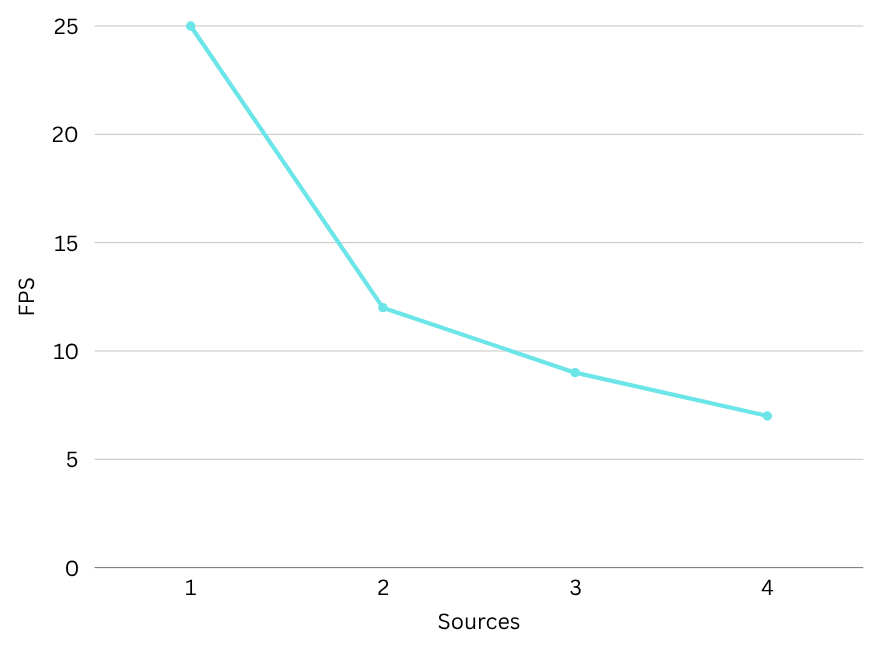
\includegraphics[width=1\linewidth]{experiment/images/pipeline_chart.png}
    \caption{Test result}
    \label{fig:enter-label}
\end{figure}
With a single input stream, the system achieved an average processing rate of 25 FPS. When the number of concurrent streams was increased to two, the average FPS per stream dropped to 12 FPS. Further increasing the load to three streams resulted in an average of 9 FPS per stream, and with four streams, the performance decreased to 7 FPS per stream.
This non-linear decrease in per-stream FPS highlights the computational limitations of the Jetson device when handling multiple high-resolution streams concurrently with the specified people counting model. While the total number of frames processed by the system per second shows a slight increase initially (1 stream: 25 total FPS; 2 streams: 24 total FPS; 3 streams: 27 total FPS; 4 streams: 28 total FPS), the quality of service for each individual stream (i.e., its fluidity and real-time nature) significantly degrades.
\begin{figure}[H]
    \centering
    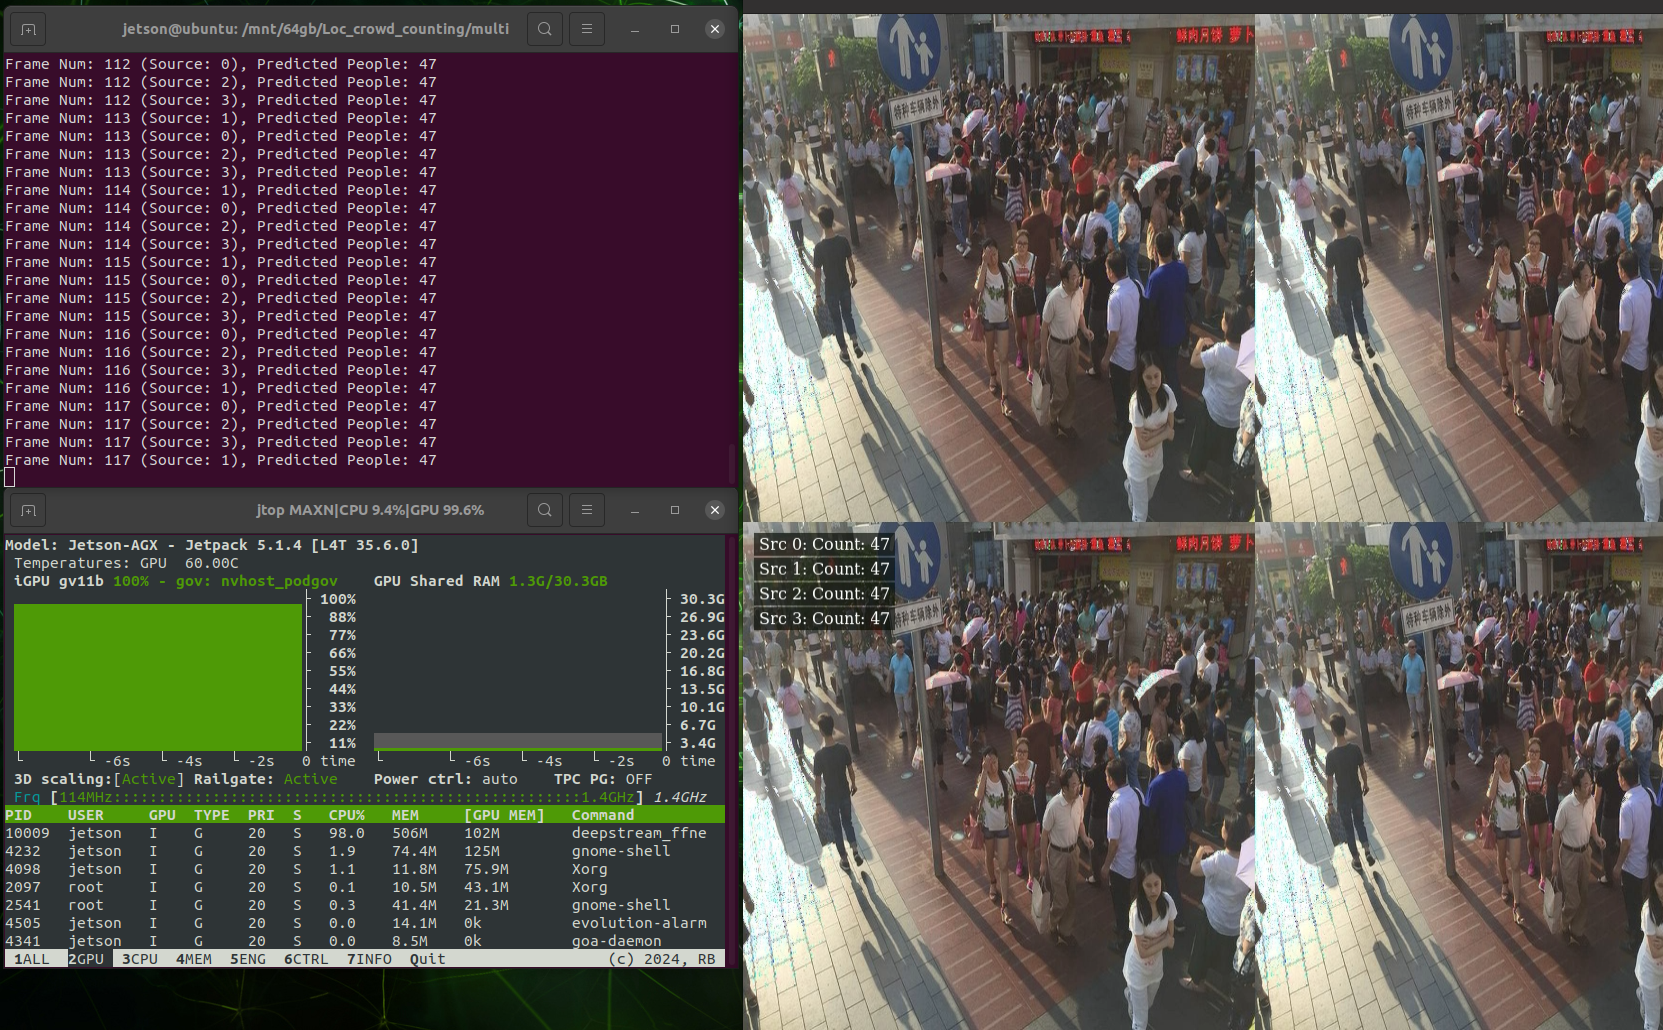
\includegraphics[width=1\linewidth]{experiment/images/pipeline_gpu.png}
    \caption{Simulation Result}
    \label{fig:enter-label}
\end{figure}

